%        File: arfc-beamer.tex
%     Created: Sun May 5 10:00 PM 2013 C


%\documentclass[11pt,handout]{beamer}
\documentclass[9pt]{beamer}
\usetheme[white]{Illinois}
%\title[short title]{long title}
\title[Research Summary]{Modeling Pyroprocessing Safeguards in Cyclus}
%\subtitle[short subtitle]{long subtitle}
\subtitle[Brief Summary]{A Brief Summary}
%\author[short name]{long name}
\author[ARFC]{Advanced Reactors and Fuel Cycles Group}
%\date[short date]{long date}
\date[09.05.2019]{January 28, 2020}
%\institution[short name]{long name}
\institute[UIUC]{University of Illinois at Urbana-Champaign}

%\usepackage{bbding}
\usepackage{amsfonts}
\usepackage{amsmath}
\usepackage{xspace}
\usepackage{graphicx}
\usepackage{subfigure}
\usepackage{booktabs} % nice rules for tables
\usepackage{microtype} % if using PDF
\usepackage{bigints}
\usepackage{tikz}
\usetikzlibrary{positioning, arrows, decorations, shapes}
\definecolor{illiniblue}{HTML}{B1C6E2}
\definecolor{illiniorange}{HTML}{f8c2a2}
\usetikzlibrary{shapes.geometric, arrows}
\tikzstyle{oblock} = [rectangle, draw, fill=illiniorange,
text width=15em, text centered, rounded corners, minimum height=4em]
\tikzstyle{bblock} = [rectangle, draw, fill=illiniblue,
text width=15em, text centered, rounded corners, minimum height=4em]
\tikzstyle{arrow} = [thick,->,>=stealth]

\usepackage{tabularx}
\newcolumntype{b}{>{\hsize=1.0\hsize}X}
\newcolumntype{s}{>{\hsize=.5\hsize}X}
\newcolumntype{m}{>{\hsize=.75\hsize}X}
\newcolumntype{x}{>{\hsize=.25\hsize}X}
\newcolumntype{L}{>{\raggedright\arraybackslash}X}
\newcolumntype{R}{>{\raggedleft\arraybackslash}X}
\def\arraystretch{1}

\newcommand{\Cyclus}{\textsc{Cyclus}\xspace}%
\newcommand{\Cycamore}{\textsc{Cycamore}\xspace}%
\newcommand{\deploy}{\texttt{d3ploy}\xspace}%
\newcommand{\units}[1] {\:\text{#1}}%
\newcommand{\SN}{S$_N$}%{S$_\text{N}$}%{$S_N$}%
\DeclareMathOperator{\erf}{erf}
%I need some complimentary error funcitons...
\DeclareMathOperator{\erfc}{erfc}
%Those icons in the references are terrible looking
\setbeamertemplate{bibliography item}[text]

\usepackage{multirow}
\usepackage{graphicx,subfigure}

%%%% Acronym support

\usepackage[acronym,toc]{glossaries}
%\newacronym{<++>}{<++>}{<++>}
\newacronym[longplural={metric tons of heavy metal}]{MTHM}{MTHM}{metric ton of heavy metal}
\newacronym{ABM}{ABM}{agent-based modeling}
\newacronym{ACDIS}{ACDIS}{Program in Arms Control \& Domestic and International Security}
\newacronym{AHTR}{AHTR}{Advanced High Temperature Reactor}
\newacronym{ANDRA}{ANDRA}{Agence Nationale pour la gestion des D\'echets RAdioactifs, the French National Agency for Radioactive Waste Management}
\newacronym{ANL}{ANL}{Argonne National Laboratory}
\newacronym{API}{API}{application programming interface}
\newacronym{ARE}{ARE}{Aircraft Reactor Experiment}
\newacronym{ARFC}{ARFC}{Advanced Reactors and Fuel Cycles}
\newacronym{ASME}{ASME}{American Society of Mechanical Engineers}
\newacronym{ATWS}{ATWS}{Anticipated Transient Without Scram}
\newacronym{BDBE}{BDBE}{Beyond Design Basis Event}
\newacronym{BIDS}{BIDS}{Berkeley Institute for Data Science}
\newacronym{CAFCA}{CAFCA}{ Code for Advanced Fuel Cycles Assessment }
\newacronym{CDTN}{CDTN}{Centro de Desenvolvimento da Tecnologia Nuclear}
\newacronym{CEA}{CEA}{Commissariat \`a l'\'Energie Atomique et aux \'Energies Alternatives}
\newacronym{CI}{CI}{continuous integration}
\newacronym{CNEN}{CNEN}{Comiss\~{a}o Nacional de Energia Nuclear}
\newacronym{CNERG}{CNERG}{Computational Nuclear Engineering Research Group}
\newacronym{COSI}{COSI}{Commelini-Sicard}
\newacronym{COTS}{COTS}{commercial, off-the-shelf}
\newacronym{CSNF}{CSNF}{commercial spent nuclear fuel}
\newacronym{CTAH}{CTAHs}{Coiled Tube Air Heaters}
\newacronym{CUBIT}{CUBIT}{CUBIT Geometry and Mesh Generation Toolkit}
\newacronym{CURIE}{CURIE}{Centralized Used Fuel Resource for Information Exchange}
\newacronym{DAG}{DAG}{directed acyclic graph}
\newacronym{DANESS}{DANESS}{Dynamic Analysis of Nuclear Energy System Strategies}
\newacronym{DBE}{DBE}{Design Basis Event}
\newacronym{DESAE}{DESAE}{Dynamic Analysis of Nuclear Energy Systems Strategies}
\newacronym{DHS}{DHS}{Department of Homeland Security}
\newacronym{DOE}{DOE}{Department of Energy}
\newacronym{DRACS}{DRACS}{Direct Reactor Auxiliary Cooling System}
\newacronym{DRE}{DRE}{dynamic resource exchange}
\newacronym{DSNF}{DSNF}{DOE spent nuclear fuel}
\newacronym{DYMOND}{DYMOND}{Dynamic Model of Nuclear Development }
\newacronym{EBS}{EBS}{Engineered Barrier System}
\newacronym{EDZ}{EDZ}{Excavation Disturbed Zone}
\newacronym{EIA}{EIA}{U.S. Energy Information Administration}
\newacronym{EPA}{EPA}{Environmental Protection Agency}
\newacronym{EP}{EP}{Engineering Physics}
\newacronym{FCO}{FCO}{Fuel Cycle Options}
\newacronym{FCT}{FCT}{Fuel Cycle Technology}
\newacronym{FEHM}{FEHM}{Finite Element Heat and Mass Transfer}
\newacronym{FEPs}{FEPs}{Features, Events, and Processes}
\newacronym{FHR}{FHR}{Fluoride-Salt-Cooled High-Temperature Reactor}
\newacronym{FLiBe}{FLiBe}{Fluoride-Lithium-Beryllium}
\newacronym{GDSE}{GDSE}{Generic Disposal System Environment}
\newacronym{GDSM}{GDSM}{Generic Disposal System Model}
\newacronym{GENIUSv1}{GENIUSv1}{Global Evaluation of Nuclear Infrastructure Utilization Scenarios, Version 1}
\newacronym{GENIUSv2}{GENIUSv2}{Global Evaluation of Nuclear Infrastructure Utilization Scenarios, Version 2}
\newacronym{GENIUS}{GENIUS}{Global Evaluation of Nuclear Infrastructure Utilization Scenarios}
\newacronym{GPAM}{GPAM}{Generic Performance Assessment Model}
\newacronym{GRSAC}{GRSAC}{Graphite Reactor Severe Accident Code}
\newacronym{GUI}{GUI}{graphical user interface}
\newacronym{HLW}{HLW}{high level waste}
\newacronym{HPC}{HPC}{high-performance computing}
\newacronym{HTC}{HTC}{high-throughput computing}
\newacronym{HTGR}{HTGR}{High Temperature Gas-Cooled Reactor}
\newacronym{IAEA}{IAEA}{International Atomic Energy Agency}
\newacronym{IEMA}{IEMA}{Illinois Emergency Mangament Agency}
\newacronym{INL}{INL}{Idaho National Laboratory}
\newacronym{IPRR1}{IRP-R1}{Instituto de Pesquisas Radioativas Reator 1}
\newacronym{IRP}{IRP}{Integrated Research Project}
\newacronym{ISFSI}{ISFSI}{Independent Spent Fuel Storage Installation}
\newacronym{ISRG}{ISRG}{Independent Student Research Group}
\newacronym{JFNK}{JFNK}{Jacobian-Free Newton Krylov}
\newacronym{LANL}{LANL}{Los Alamos National Laboratory}
\newacronym{LBNL}{LBNL}{Lawrence Berkeley National Laboratory}
\newacronym{LCOE}{LCOE}{levelized cost of electricity}
\newacronym{LDRD}{LDRD}{laboratory directed research and development}
\newacronym{LFR}{LFR}{Lead-Cooled Fast Reactor}
\newacronym{LLNL}{LLNL}{Lawrence Livermore National Laboratory}
\newacronym{LMFBR}{LMFBR}{Liquid Metal Fast Breeder Reactor}
\newacronym{LOFC}{LOFC}{Loss of Forced Cooling}
\newacronym{LOHS}{LOHS}{Loss of Heat Sink}
\newacronym{LOLA}{LOLA}{Loss of Large Area}
\newacronym{LP}{LP}{linear program}
\newacronym{LWR}{LWR}{Light Water Reactor}
\newacronym{MA}{MA}{minor actinide}
\newacronym{MCNP}{MCNP}{Monte Carlo N-Particle code}
\newacronym{MILP}{MILP}{mixed-integer linear program}
\newacronym{MIT}{MIT}{the Massachusetts Institute of Technology}
\newacronym{MOAB}{MOAB}{Mesh-Oriented datABase}
\newacronym{MOOSE}{MOOSE}{Multiphysics Object-Oriented Simulation Environment}
\newacronym{MOX}{MOX}{mixed oxide}
\newacronym{MSBR}{MSBR}{Molten Salt Breeder Reactor}
\newacronym{MSRE}{MSRE}{Molten Salt Reactor Experiment}
\newacronym{MSR}{MSR}{Molten Salt Reactor}
\newacronym{NAGRA}{NAGRA}{National Cooperative for the Disposal of Radioactive Waste}
\newacronym{NEAMS}{NEAMS}{Nuclear Engineering Advanced Modeling and Simulation}
\newacronym{NEUP}{NEUP}{Nuclear Energy University Programs}
\newacronym{NFCSim}{NFCSim}{Nuclear Fuel Cycle Simulator}
\newacronym{NGNP}{NGNP}{Next Generation Nuclear Plant}
\newacronym{NMWPC}{NMWPC}{Nuclear MW Per Capita}
\newacronym{NNSA}{NNSA}{National Nuclear Security Administration}
\newacronym{NPRE}{NPRE}{Department of Nuclear, Plasma, and Radiological Engineering}
\newacronym{NQA1}{NQA-1}{Nuclear Quality Assurance - 1}
\newacronym{NRC}{NRC}{Nuclear Regulatory Commission}
\newacronym{NSF}{NSF}{National Science Foundation}
\newacronym{NSSC}{NSSC}{Nuclear Science and Security Consortium}
\newacronym{NUWASTE}{NUWASTE}{Nuclear Waste Assessment System for Technical Evaluation}
\newacronym{NWF}{NWF}{Nuclear Waste Fund}
\newacronym{NWTRB}{NWTRB}{Nuclear Waste Technical Review Board}
\newacronym{OCRWM}{OCRWM}{Office of Civilian Radioactive Waste Management}
\newacronym{ORION}{ORION}{ORION}
\newacronym{ORNL}{ORNL}{Oak Ridge National Laboratory}
\newacronym{PARCS}{PARCS}{Purdue Advanced Reactor Core Simulator}
\newacronym{PBAHTR}{PB-AHTR}{Pebble Bed Advanced High Temperature Reactor}
\newacronym{PBFHR}{PB-FHR}{Pebble-Bed Fluoride-Salt-Cooled High-Temperature Reactor}
\newacronym{PEI}{PEI}{Peak Environmental Impact}
\newacronym{PH}{PRONGHORN}{PRONGHORN}
\newacronym{PRKE}{PRKE}{Point Reactor Kinetics Equations}
\newacronym{PSPG}{PSPG}{Pressure-Stabilizing/Petrov-Galerkin}
\newacronym{PWAR}{PWAR}{Pratt and Whitney Aircraft Reactor}
\newacronym{PWR}{PWR}{Pressurized Water Reactor}
\newacronym{PyNE}{PyNE}{Python toolkit for Nuclear Engineering}
\newacronym{PyRK}{PyRK}{Python for Reactor Kinetics}
\newacronym{QA}{QA}{quality assurance}
\newacronym{RDD}{RD\&D}{Research Development and Demonstration}
\newacronym{RD}{R\&D}{Research and Development}
\newacronym{RELAP}{RELAP}{Reactor Excursion and Leak Analysis Program}
\newacronym{RIA}{RIA}{Reactivity Insertion Accident}
\newacronym{RIF}{RIF}{Region-Institution-Facility}
\newacronym{SFR}{SFR}{Sodium-Cooled Fast Reactor}
\newacronym{SINDAG}{SINDA{\textbackslash}G}{Systems Improved Numerical Differencing Analyzer $\backslash$ Gaski}
\newacronym{SKB}{SKB}{Svensk K\"{a}rnbr\"{a}nslehantering AB}
\newacronym{SNF}{SNF}{spent nuclear fuel}
\newacronym{SNL}{SNL}{Sandia National Laboratory}
\newacronym{STC}{STC}{specific temperature change}
\newacronym{SUPG}{SUPG}{Streamline-Upwind/Petrov-Galerkin}
\newacronym{SWF}{SWF}{Separations and Waste Forms}
\newacronym{SWU}{SWU}{Separative Work Unit}
\newacronym{TRIGA}{TRIGA}{Training Research Isotope General Atomic}
\newacronym{TRISO}{TRISO}{Tristructural Isotropic}
\newacronym{TSM}{TSM}{Total System Model}
\newacronym{TSPA}{TSPA}{Total System Performance Assessment for the Yucca Mountain License Application}
\newacronym{ThOX}{ThOX}{thorium oxide}
\newacronym{UFD}{UFD}{Used Fuel Disposition}
\newacronym{UML}{UML}{Unified Modeling Language}
\newacronym{UOX}{UOX}{uranium oxide}
\newacronym{UQ}{UQ}{uncertainty quantification}
\newacronym{US}{US}{United States}
\newacronym{UW}{UW}{University of Wisconsin}
\newacronym{VISION}{VISION}{the Verifiable Fuel Cycle Simulation Model}
\newacronym{VV}{V\&V}{verification and validation}
\newacronym{WIPP}{WIPP}{Waste Isolation Pilot Plant}
\newacronym{YMR}{YMR}{Yucca Mountain Repository Site}


\makeglossaries

%try to get rid of header on title page\dots
\makeatletter
    \newenvironment{withoutheadline}{
        \setbeamertemplate{headline}[default]
        \def\beamer@entrycode{\vspace*{-\headheight}}
    }{}
\makeatother

\makeatother
\setbeamertemplate{footline}
{
  \leavevmode%
  \hbox{%
    \rightline{\insertframenumber{} / \inserttotalframenumber\hspace*{1ex}}
  }%
  \vskip0pt%
}
\makeatletter
\begin{document}
%%%%%%%%%%%%%%%%%%%%%%%%%%%%%%%%%%%%%%%%%%%%%%%%%%%%%%%%%%%%%
%% From uw-beamer Here's a handy bit of code to place at 
%% the beginning of your presentation (after \begin{document}):
\newcommand*{\alphabet}{ABCDEFGHIJKLMNOPQRSTUVWXYZabcdefghijklmnopqrstuvwxyz}
\newlength{\highlightheight}
\newlength{\highlightdepth}
\newlength{\highlightmargin}
\setlength{\highlightmargin}{2pt}
\settoheight{\highlightheight}{\alphabet}
\settodepth{\highlightdepth}{\alphabet}
\addtolength{\highlightheight}{\highlightmargin}
\addtolength{\highlightdepth}{\highlightmargin}
\addtolength{\highlightheight}{\highlightdepth}
\newcommand*{\Highlight}{\rlap{\textcolor{HighlightBackground}{\rule[-\highlightdepth]{\linewidth}{\highlightheight}}}}
%%%%%%%%%%%%%%%%%%%%%%%%%%%%%%%%%%%%%%%%%%%%%%%%%%%%%%%%%%%%%
%%--------------------------------%%
\begin{withoutheadline}
\frame{
  \titlepage
}
\end{withoutheadline}

%%--------------------------------%%
\AtBeginSection[]{
\begin{frame}
  \frametitle{Outline}
  \tableofcontents[currentsection]
\end{frame}
}

\section{Background}
\begin{frame}
	\frametitle{Education}
	\begin{columns}
		\column[t]{5cm}
		\begin{figure}
			
\includegraphics[width=0.7\linewidth]{mst}
		\end{figure}
		\begin{figure}
		
\includegraphics[width=\linewidth]{uiuc}
		\end{figure}
		\column[t]{6cm}
		\begin{figure}
		
\includegraphics[width=0.7\linewidth]{wustl}
		\end{figure}
	\end{columns}
\end{frame}

\begin{frame}
\frametitle{Washington University}
\begin{columns}
	\column[t]{5cm}
	\begin{figure}
		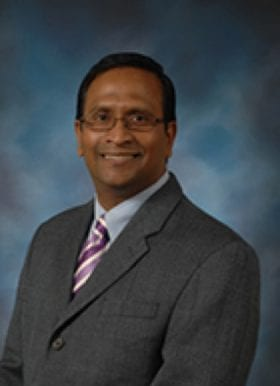
\includegraphics[width=0.7\linewidth]{goddu}
		\caption{Dr. S. Murty Goddu - Radiation Oncology}
	\end{figure}
	\column[t]{6cm}
	\begin{figure}
		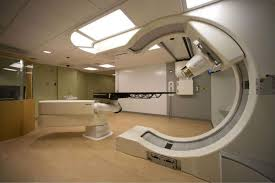
\includegraphics[width=\linewidth]{proton}
		\caption{Washington University's Proton Therapy}
	\end{figure}
\end{columns}
\end{frame}

\begin{frame}
\frametitle{CNEC - UIUC}
\begin{columns}
	\column[t]{5cm}
	\begin{figure}
		
\includegraphics[width=\linewidth]{cnec}
	\end{figure}
	\begin{itemize}
		\item NNSA funded consortia:
		\begin{itemize}
			\item Frequent workshops/conferences.
			\item Lab interaction.
		\end{itemize}
		\item IAEA NDA training:
		\begin{itemize}
			\item Introduction to NDA techniques.
			\item Safeguard applications - UNCL.
		\end{itemize}
		\item Software Development - Cyclus
	\end{itemize}
	\column[t]{6cm}
	\begin{figure}
		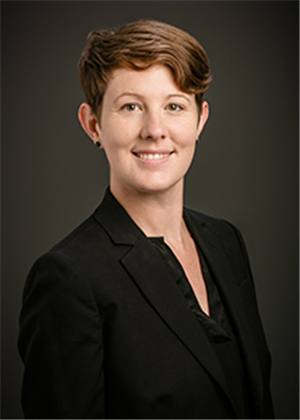
\includegraphics[width=0.6\linewidth]{katy}
		\caption{Professor Katy Huff}
	\end{figure}
\end{columns}
\end{frame}
\section{Introduction}
\begin{frame}
\frametitle{Introduction}
	\begin{figure}
		\centering
		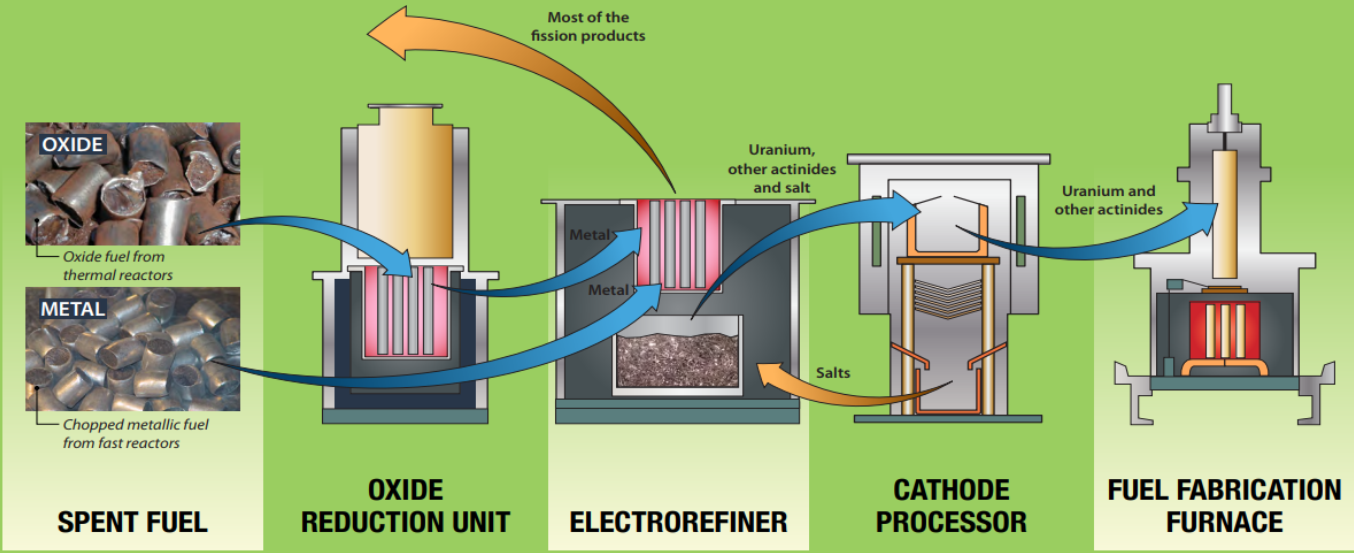
\includegraphics[width=\linewidth]{pyro-background.png}
		\caption{Argonne demonstration of a basic pyro plant \cite{williamson_pyroprocessing_nodate}.}
		\label{fig:pyro}
	\end{figure}
\end{frame}

\begin{frame}
\frametitle{Motivation/Goals}
\textbf{Motivation}
\begin{itemize}
	\item Safeguard by design
	\item Model diversion inside facilities
	\item Transition from LWR to SFR
\end{itemize}
\textbf{Goals}
\begin{itemize}
	\item Detect diversion using signatures and observables.
	\item Determine optimum detector and inspection locations in pyroprocessing
	\item Characterize detection sensitivities
\end{itemize}
\end{frame}


\begin{frame}
\frametitle{Inspiration}
\begin{figure}
\centering

\includegraphics[width=0.9\linewidth]{borrelli-citation.png}
\end{figure}
\end{frame}
\section{Methods}
\begin{frame}
\frametitle{Assumptions}
\begin{columns}
	\begin{column}{.55\textwidth}
		\begin{block}{Cyclus Requirements} 
			\begin{itemize}
				\item Modular.
				\item Time step $\geq$ 1 month
				\item Streams must be in a
				trade-able form.
				\item Parameters are constant for the simulation.
				\begin{itemize}
					\item Equation input toolkit under development.
				\end{itemize}
				\item Diversion detection must be added after.
			\end{itemize}
		\end{block}
	\end{column}
	\begin{column}{.45\textwidth}
		\begin{figure}
			\centering
			
\includegraphics[width=0.9\linewidth]{cyclus}
			\label{fig:cyclus}
		\end{figure}
	\end{column}
\end{columns} 
\end{frame}

\begin{frame}
\frametitle{Subprocesses - Voloxidation}
		\begin{figure} 
			\centering
			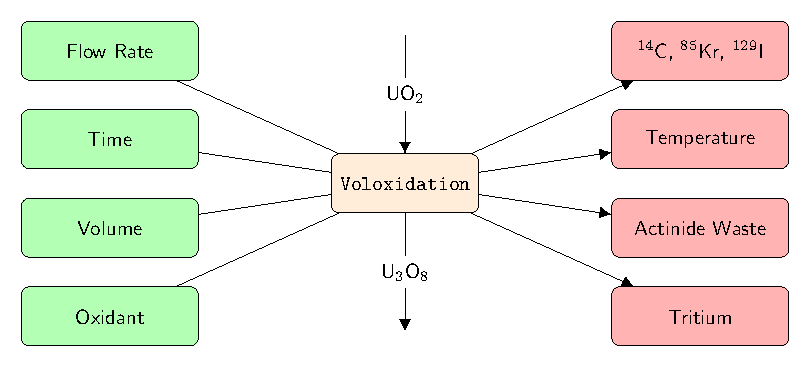
\includegraphics[width=0.9\linewidth]{volox}
			\caption{Voloxidation material balance area \cite{jubin_spent_2009}.}
			\label{fig:volox}
		\end{figure}
\end{frame}
\begin{frame}
\frametitle{Subprocesses - Electroreduction}
		\begin{figure} 
			\centering
			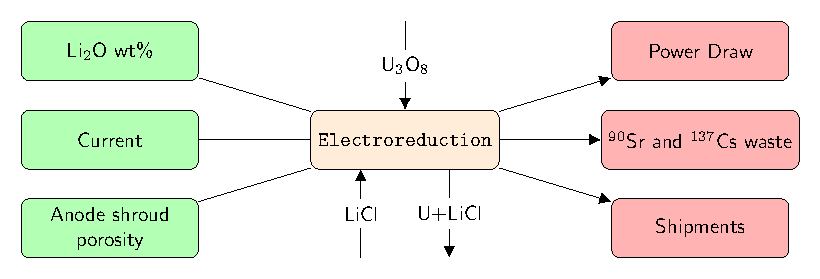
\includegraphics[width=0.9\linewidth]{reduction}
			\caption{Reduction material balance area \cite{lee_advanced_2008}.}
			\label{fig:reduction}
		\end{figure}
\end{frame}
\begin{frame}
\frametitle{Subprocesses - Electrorefining}
		\begin{figure}
			\centering
			\includegraphics[width=0.85\linewidth]{refining}
			\caption{Refining material balance area \cite{lee_advanced_2008}.}
			\label{fig:refining}
		\end{figure}
\end{frame}
\begin{frame}
\frametitle{Subprocesses - Electrowinning}
		\begin{figure} 
			\centering
			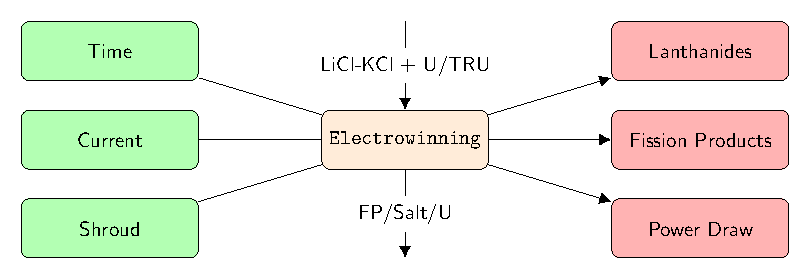
\includegraphics[width=0.8\linewidth]{winning}
			\caption{Winning material balance area.}
			\label{fig:winning}
		\end{figure}
\end{frame}
\section{Pyre}
\begin{frame}
	\frametitle{Pyre Archetype}
	\begin{columns}
		\column[t]{5cm}
		\begin{itemize}
			\item Facility containing multiple sub-processes:
			\begin{itemize}
				\item Separately handled.
				\item Independent transactions, possibility of diversion.
			\end{itemize}
			\item Operation setting impact efficiency.
			\item Generic facility:
			\begin{itemize}
				\item Multiple types of pyro plants.
				\item LWR vs SFR.
			\end{itemize}
		\end{itemize}
		\column[t]{6cm}
		\begin{figure}
			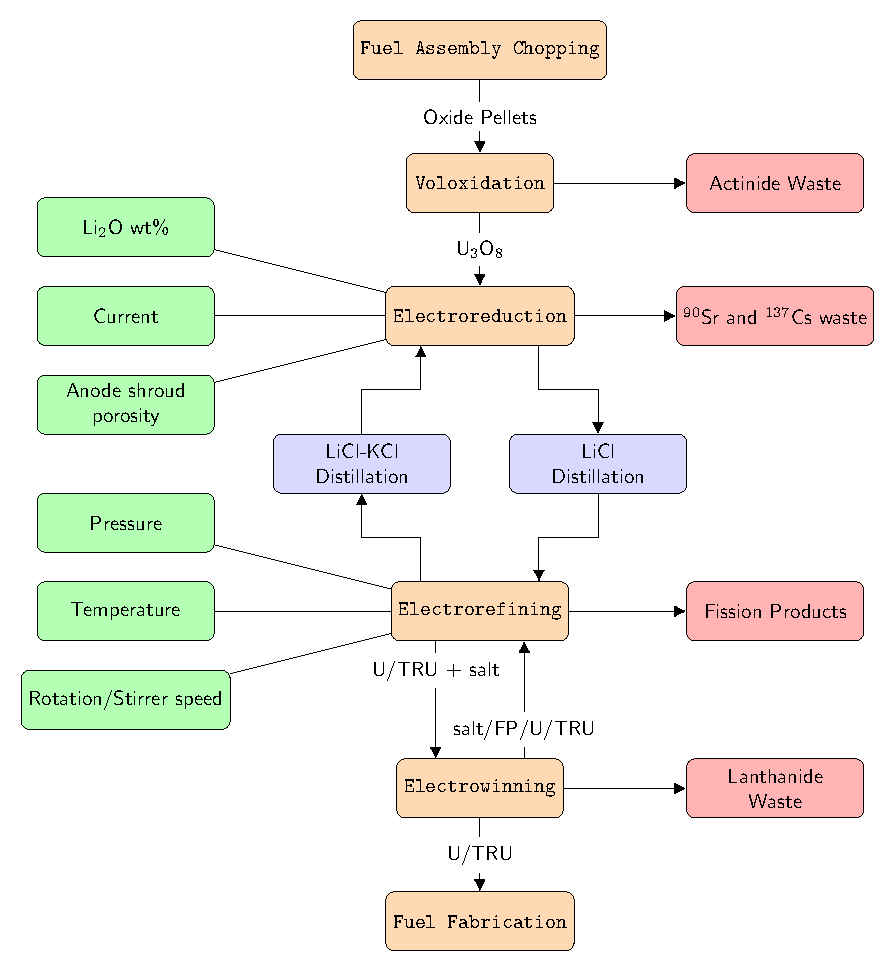
\includegraphics[width=\linewidth]{./images/westphal-pyre.pdf}
			\caption{PyRe flow diagram for LWR waste configuration.}
			\label{fig:pyre}
		\end{figure}
	\end{columns}
\end{frame}

\begin{frame}
\frametitle{Pyre - Diversion Options}
Material diversion occurs in two different modes: \textbf{nefarious} or \textbf{operator}.
\begin{itemize}
	\item \textbf{Nefarious Diversion} imagines diversion by a single bad actor with facility access.
	\item \textbf{Operator Diversion} imagines undeclared production.
\end{itemize}
\begin{figure}
	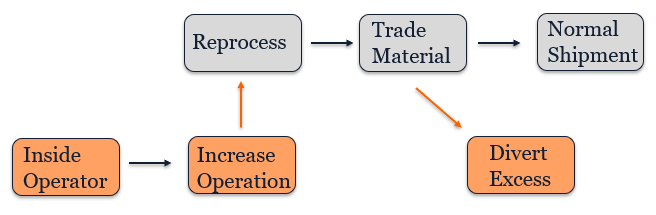
\includegraphics[width=0.7\linewidth]{./images/westphal-diversion}
	\caption{Operator vs nefarious diversion.}
	\label{fig:diversion}
\end{figure}
\end{frame}

\begin{frame}
	\frametitle{Diverter Class}
	\begin{columns}
		\column[t]{5cm}
		Inputs:
		\begin{itemize}
			\item Location
			\begin{itemize}
				\item Sub-process
				\item Operation Setting
			\end{itemize}
			\item Quantity
			\item Frequency
			\item Number of Diversions
		\end{itemize}
		\begin{block}{Purpose}
			The goal of a separate diverter class is to allow this method to be used by facilities other
			than pyre through a toolkit.
		\end{block}
		\column[t]{6cm}
		\begin{figure}
			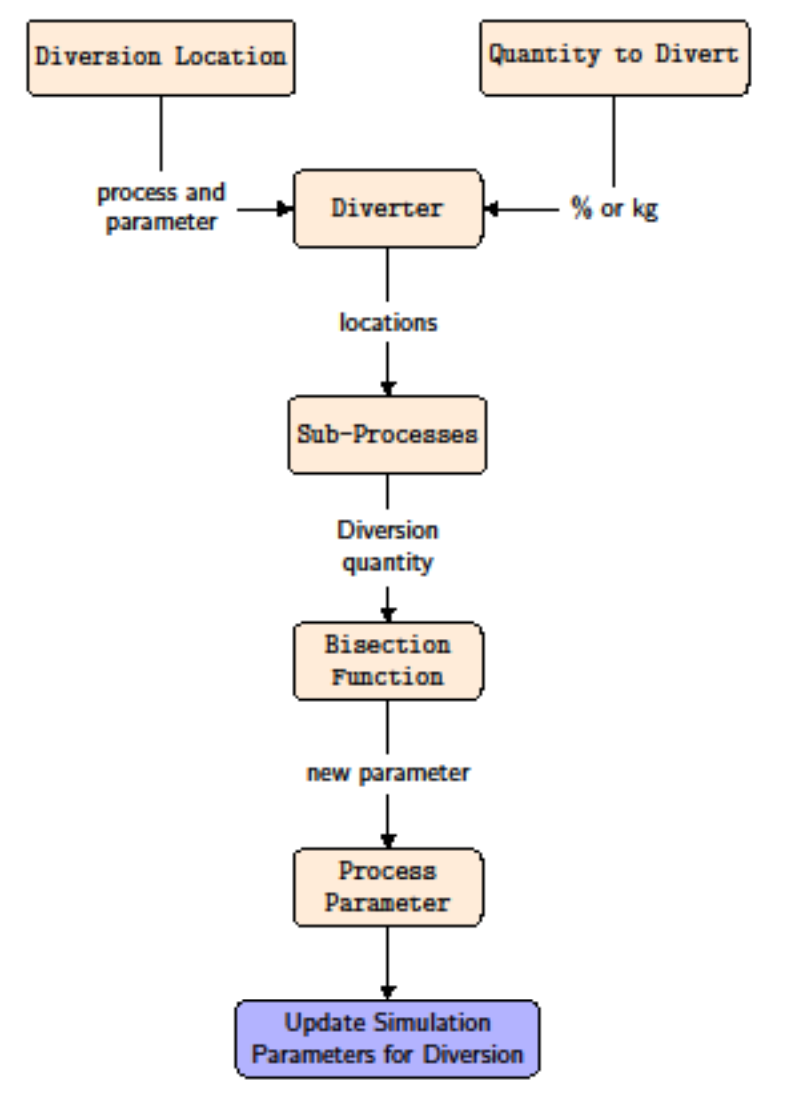
\includegraphics[width=0.8\linewidth]{images/diverter}
			\label{fig:diverter}
		\end{figure}
	\end{columns}
\end{frame}

\begin{frame}
\frametitle{Diversion Detection}
\begin{columns}
	\column[t]{5cm}
	\begin{block}{Diversion Detection}
		Material transactions are no longer a reliable method. Instead we use
		signatures and observables:
		\begin{itemize}
			\item Temperature, power draw, etc.
		\end{itemize}
		A Cumulative Sum change algorithm is used to detect any significant changes.
	\end{block}
	\column[t]{6cm}
	\begin{figure}
		\includegraphics[width=\linewidth]{images/refining}
	\end{figure}
\end{columns}
\end{frame}

\begin{frame}
\frametitle{Transition Scenario}
A main attraction of pyroprocessing is the ability to handle LWR and
SFR waste.
\begin{itemize}
	\item To verify this capability in PyRe, we ran an EG01 – EG24 transition
	scenario.
	\item We want to observe the following:
	\begin{itemize}
		\item Appropriate deploying of PyRe
		\item Ability to meet demand of new SFRs
		\item Diversion capabilities
		\item Accurate transition from UOX to SFR fuels
	\end{itemize}
\end{itemize}
\end{frame}

\begin{frame}
\frametitle{Transition Scenario - Setup}
Legacy:
\begin{itemize}
	\item 200 LWRs
	\begin{itemize}
		\item 50\% 60yr lifetime
		\item 50\% 80yr lifetime
	\end{itemize}
	\item LWR Pyre
\end{itemize}

Transition:
\begin{itemize}
	\item ~200 LWRs starting in 2015
	\begin{itemize}
		\item 80yr lifetime
	\end{itemize}
	\item SFR starts in 2050
	\begin{itemize}
		\item 80yr lifetime
	\end{itemize}
	\item SFR Pyre
\end{itemize}
\end{frame}

\begin{frame}
\frametitle{Transition Scenario - Results}
\begin{figure}
	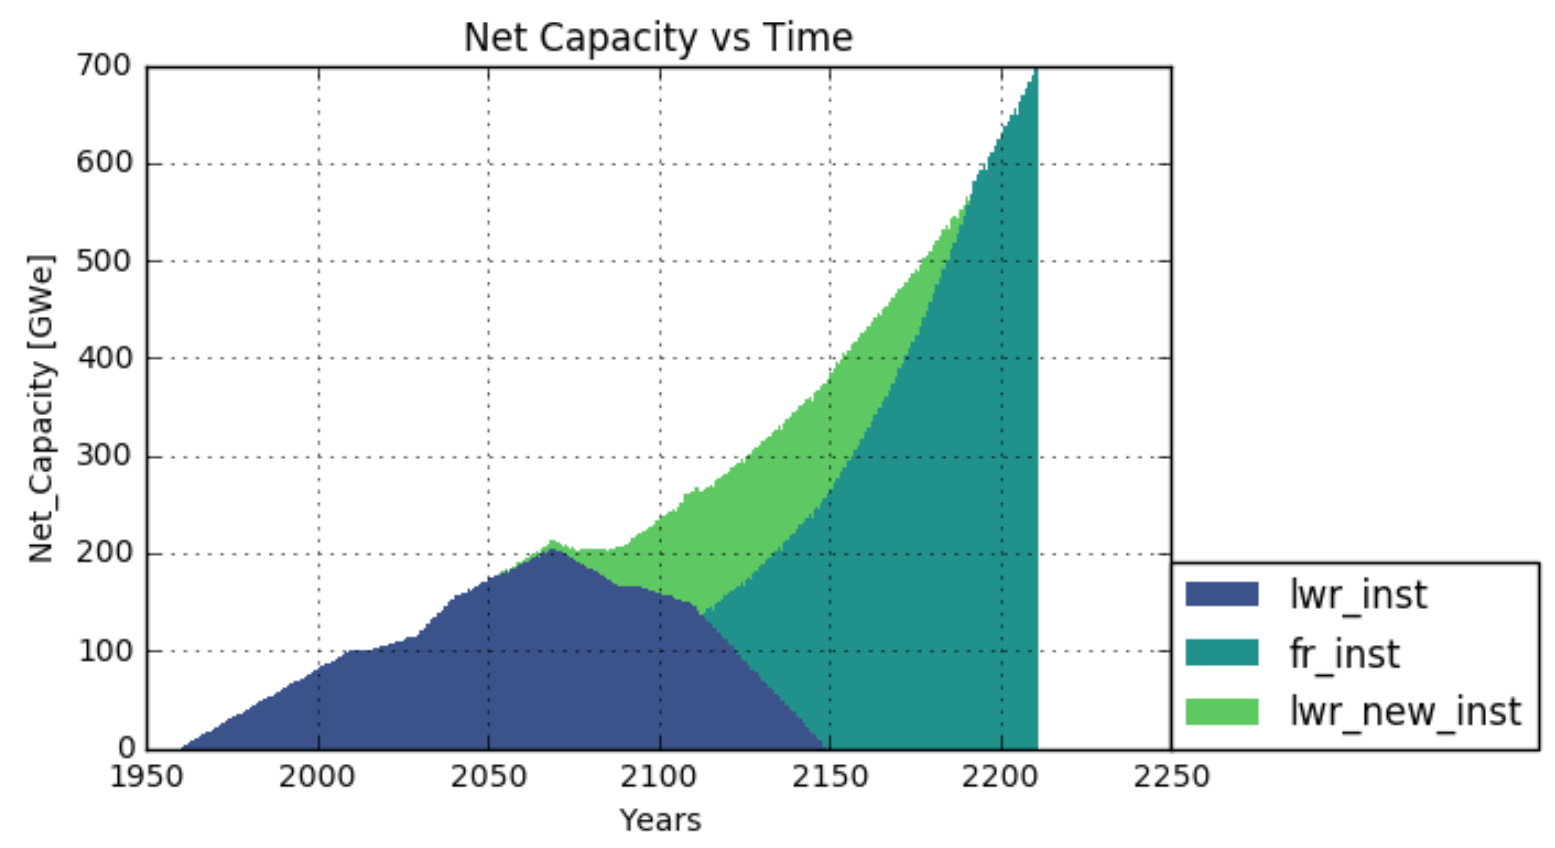
\includegraphics[width=\linewidth]{images/netcap}
\end{figure}
\end{frame}

\begin{frame}
\frametitle{Diversion Settings}
\begin{columns}
	\column[t]{4cm}
	Two Pyre prototypes:
	\begin{itemize}
		\item LWR vs SFR
	\end{itemize}
	LWR Pyre:
	\begin{itemize}
		\item Fewer diversions
		\item More material per instance
		\item Less frequent
	\end{itemize}
	SFR Pyre:
	\begin{itemize}
		\item Frequent diversion
		\item Small quantities
	\end{itemize}
	\column[t]{7cm}
	\begin{figure}
		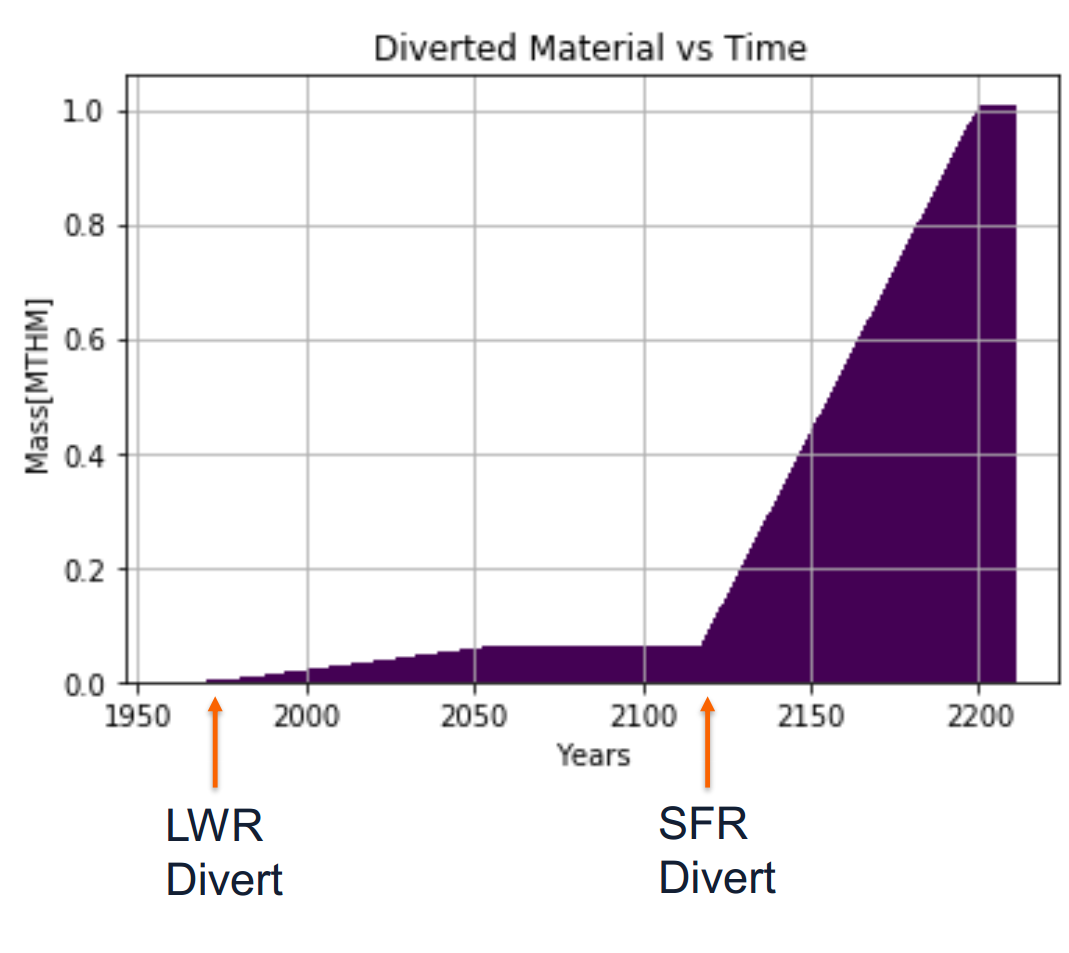
\includegraphics[width=\linewidth]{images/divertmat}
	\end{figure}
\end{columns}
\end{frame}

\begin{frame}
\frametitle{Transition Scenario - Utilization}
\begin{figure}
	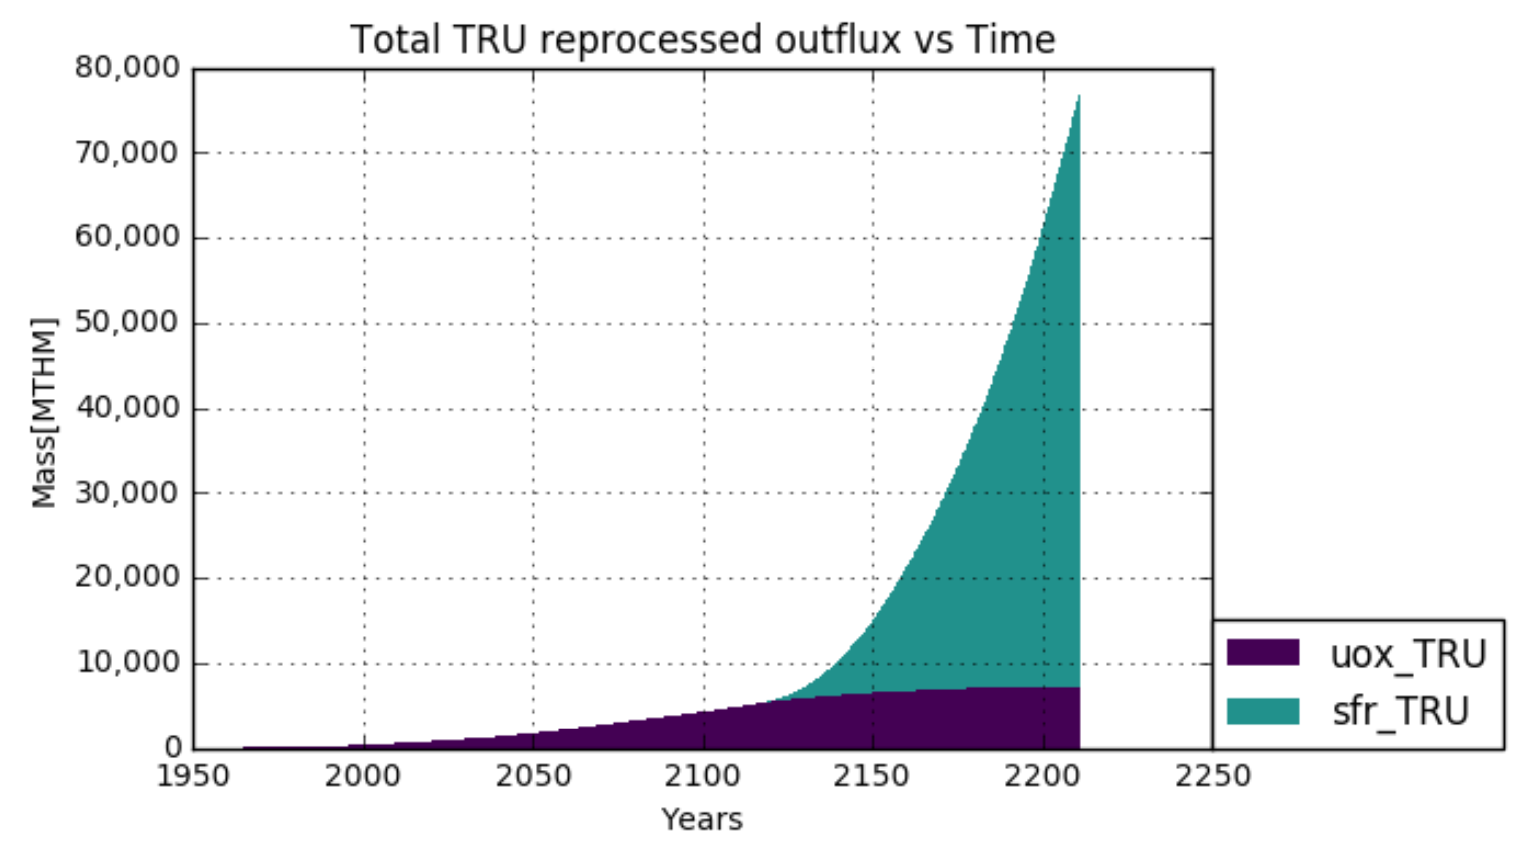
\includegraphics[width=\linewidth]{images/truutil}
\end{figure}
\end{frame}

\begin{frame}
\frametitle{Transition Scenario - Utilization}
\begin{figure}
	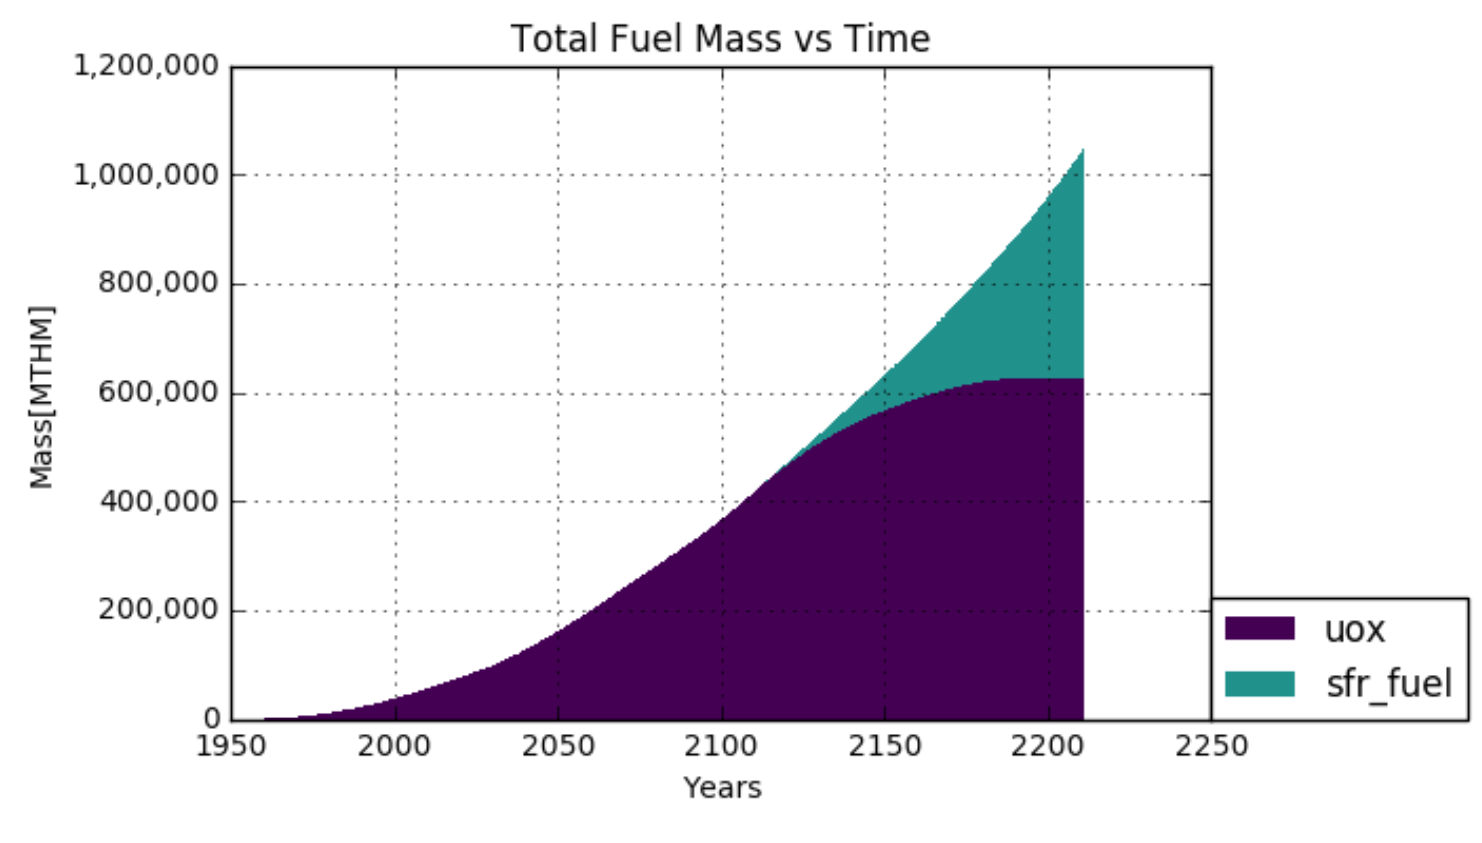
\includegraphics[width=\linewidth]{images/fuelmass}
\end{figure}
\end{frame}

\begin{frame}
\frametitle{Conclusions}
We have developed a customizable method of diverting material
from inside Cyclus facilities.
\begin{itemize}
	\item Preliminary work has been done on the detection of two
	different types of diversion: Nefarious and Operator
\end{itemize}
PyRe was demonstrated to function as both LWR and SFR
reprocessing method
\begin{itemize}
	\item Generic facility capable of modeling multiple facility layouts
\end{itemize}
\end{frame}
\section{Sensitivity}
\begin{frame}
\frametitle{Sensitivity Analysis}
Dakota was wrapped around Cyclus to randomly sample various parameters for critical sub-processes:
\begin{itemize}
	\item Electrorefiner
	\item Electrowinner
\end{itemize}

\begin{figure}
	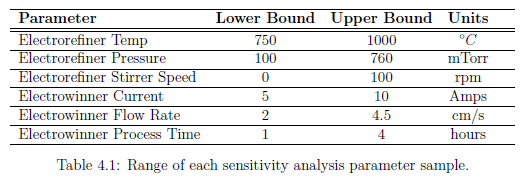
\includegraphics[width=\linewidth]{sens-params}
\end{figure}
\end{frame}

\begin{frame}
\frametitle{Electrorefiner - Temperature}
\begin{figure}
	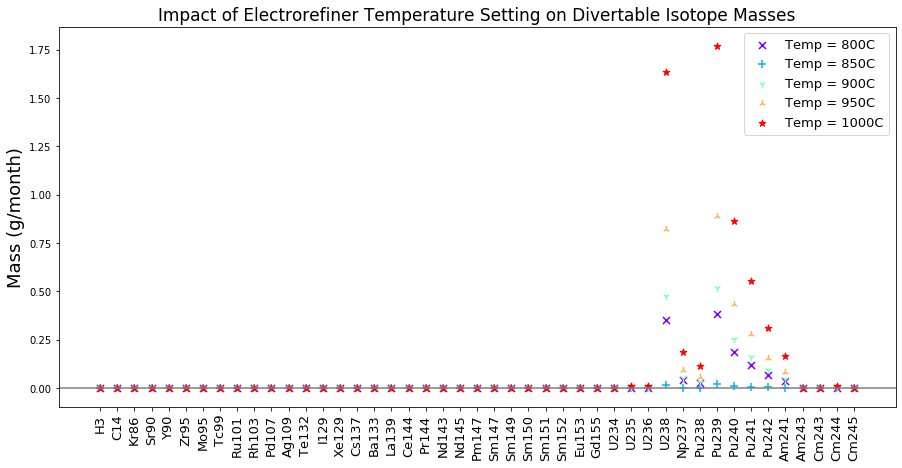
\includegraphics[width=\linewidth]{./images/temperature-sa-diff}
\end{figure}
\end{frame}

\begin{frame}
	\frametitle{Electrorefiner - Stirrer}
	\begin{figure}
		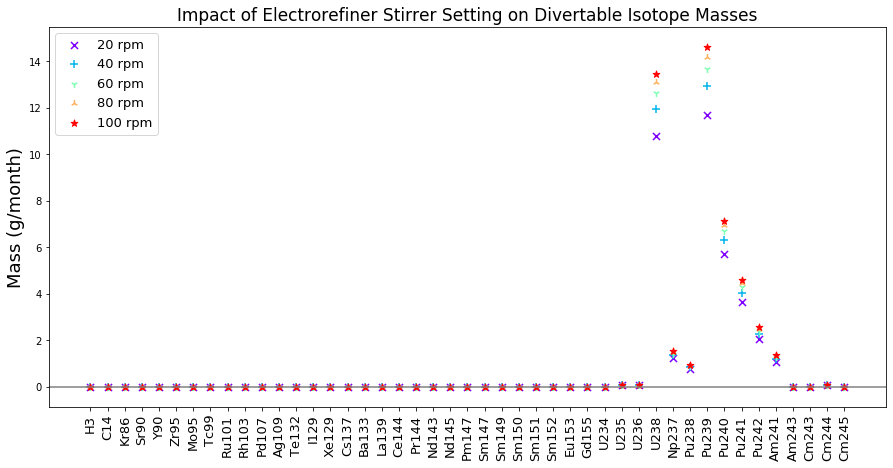
\includegraphics[width=\linewidth]{./images/rotation-sa-diff}
	\end{figure}
\end{frame}

\begin{frame}
	\frametitle{Electrowinner - Current}
	\begin{figure}
		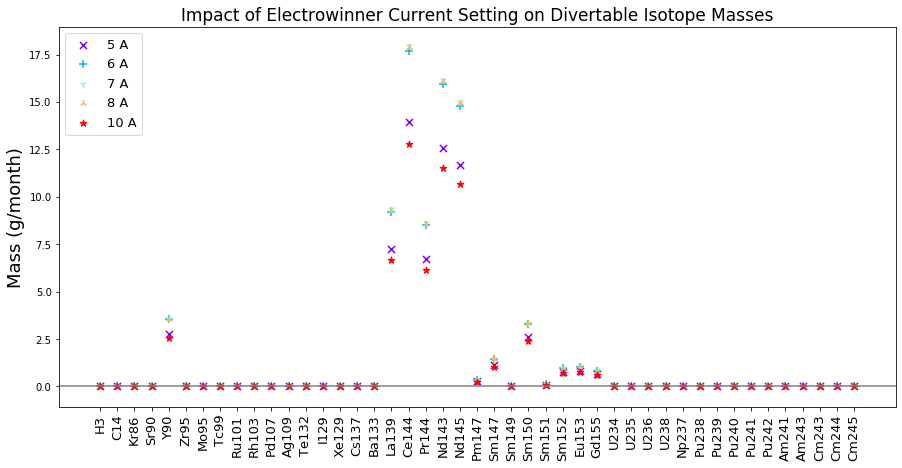
\includegraphics[width=\linewidth]{./images/current-sa-diff}
	\end{figure}
\end{frame}

\begin{frame}
	\frametitle{Electrorefiner - Process Time}
	\begin{figure}
		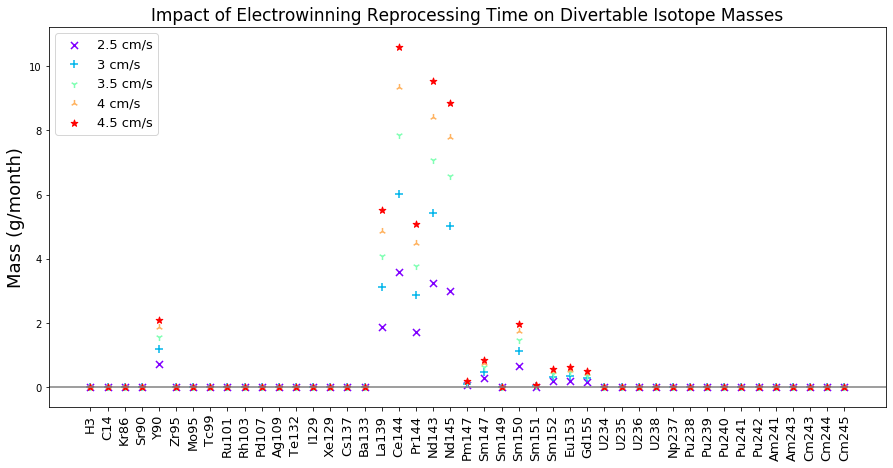
\includegraphics[width=\linewidth]{./images/time-sa-diff}
	\end{figure}
\end{frame}

\begin{frame}
\frametitle{Sensitivity Results}
	Parameters that influenced interaction between eutectic and waste showed more significant impact on separation efficiency.
	\begin{figure}
		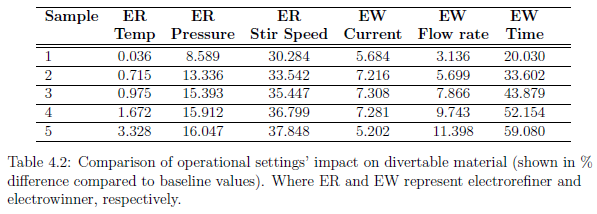
\includegraphics[width=\linewidth]{sens-results}
	\end{figure}
\end{frame}
\section{Conclusion}
\begin{frame}
\frametitle{Conclusions}
We have developed a customizable method of diverting material
from inside Cyclus facilities.
\begin{itemize}
	\item Work has been done on the detection of two
	different types of diversion: Nefarious and Operator
\end{itemize}
Pyre was demonstrated to function as both LWR and SFR
reprocessing method
\begin{itemize}
	\item Generic facility capable of modeling multiple facility layouts
\end{itemize}
Key measurement points were identified with sensitivity analysis performed over the primary sub-processes.
\end{frame}

\begin{frame}
\frametitle{Future Work}
This work laid the groundwork for future research into sub-facility modeling and diversion detection. Future additions to this work could include:
\begin{itemize}
	\item Reducing time step length for higher fidelity
	\item Expand on operational parameter relationships with further experimental data
	\item Incorporate multiple data points for CUSUM detection
\end{itemize}
\end{frame}

\section{Acknowledgments}
\begin{frame}
\frametitle{Acknowledgement}
This work is supported by U.S. Department of Energy, 
Nuclear Energy University Program, under contract 
\#NEUP-FY16-10512. 
\end{frame}


%%--------------------------------%%
%%--------------------------------%%
\begin{frame}[allowframebreaks]
  \frametitle{References}
  \bibliographystyle{plain}
  {\footnotesize \bibliography{2019-09-05-group} }
\end{frame}

%%--------------------------------%%

\end{document}

